\documentclass[11pt]{article}
\usepackage{amsmath, amssymb}
\usepackage{geometry}
\geometry{margin=1in}
\usepackage{fancyhdr}
\usepackage{lastpage}
\usepackage{parskip} % Better paragraph spacing
\usepackage{titlesec} % Better section formatting
\usepackage{graphicx}
\usepackage{float}
\usepackage[most]{tcolorbox}
\usepackage{lmodern}
\usepackage{caption}

% Define commands for reusable content
\newcommand{\coursename}{CS-401 Applied Data Analysis}
\newcommand{\lecturenum}{04}
\newcommand{\lecturedate}{\today}
\newcommand{\professor}{Maria Brbic}

% Configure section spacing
\titlespacing*{\section}{0pt}{2ex plus 1ex minus .2ex}{1.5ex plus .2ex}
% Header / Footer
\pagestyle{fancy}
\fancyhf{}
\fancyhead[L]{\coursename}
\fancyhead[R]{Lecture \lecturenum}
\fancyfoot[L]{EPFL - Computer Science}
\fancyfoot[C]{Author: Jonathan Dutoit}
\fancyfoot[R]{Page \thepage\ of \pageref{LastPage}}

\begin{document}

\begin{center}
  {\large EPFL - Computer Science} \\[0.5em]
  {\Large \textbf{\coursename}} \\[0.5em]
  {\large Lecture \lecturenum\ --- \lecturedate} \\[0.5em]
  {\large Author: Jonathan Dutoit} \\[0.5em]
  {\large Professor: \professor} \\[0.5em]
\end{center}

\vspace{2cm}

\begin{center}
  {\LARGE \textbf{Describing Data}}
\end{center}

\vspace{1cm}

\section*{Overview of today's lecture}
\begin{itemize}
	\item \textcolor{red}{Part 1}: Descriptive statistics
	\item \textcolor{red}{Part 2}: Quantifying uncertainty
	\item \textcolor{red}{Part 3:} Relating two variables
\end{itemize}

\begin{center}
  {\LARGE \textbf{Part 1}: Descriptive statistics
\end{center}

\vspace{1cm}

\section*{Robust statistics}

A statistic is said to be robust if it is not sensitive to \textbf{extreme values}

Min, max, mean, standard deviation are \textcolor{red}{not robuts}

Median, quartiles (and others) are \textcolor{blue}{robust}

\section*{Heavy-tailed distributions}

\begin{itemize}
	\item Some distributions are all about the extreme values
	\item E.g., power laws: $f(x) = ax^{-k}$ 
	\begin{itemize}
		\item Very very large values are, "but not very rare"
		\item Body size vs. city size
		\item For k <= 3: infinite variance
		\item For k <= 2: infinite variance, infinite mean
		\item Don't report (arithmetic) mean/variance for power-law-distributed data!
		\item Use robust statistics (e.g., mean, quantiles, etc.) or geometric mean
	\end{itemize}
\end{itemize}

\section*{Generalized means}
\begin{itemize}
	\item Common trick: transform data into a different space (via function \textit{f}), take mean there, then transform back into the original space (via $f^{-1}$ )
\[
	f^{-1}(\frac{1}{n} \sum_{i=1}^{n}{f(x_i)})
.\] 		
\end{itemize}

\begin{itemize}
	\item f(x) = $x^{2}$, $f^{-1}(x) = \sqrt{x}$  “root mean square”
	\item f(x) = x, $f^{-1} = x$ “arithmetic mean”
	\item f(x) = log(x), $f^{-1}$ = exp(x) "geometric mean"
	\item f(x) = 1/x, $f^{-1} = 1/x$ "harmonic mean"
\end{itemize}

\section*{Distributions}

Some important distributions:
\begin{itemize}
	\item \textbf{Normal}: see previous slides
	\item \textbf{Poisson}: the distribution of counts that occur at a certain "rate"; e.g., number of visits to a given website in a fixed time interval. 
	\item \textbf{Exponential}: the interval between two such events
	\item \textbf{Binomial/multinomial}: the number of "successes" (e.g., coin flips = heads) out of n trials
	\item \textbf{Power-law/Zipf/Pareto/Yule}: e.g., frequencies of different terms in a document; city size
\end{itemize}

\textcolor{red}{You should understand the distribution of your data before applying any model!}
\section*{"Dear data, where are you from?"}

\begin{itemize}
	\item Visual inspection for ruling out certain distributions: e.g., when histogram/box plot is asymmetric (even for large sample size), the data cannot be normal
\end{itemize}
% Quick centered image
\begin{figure}[H]
    \centering
    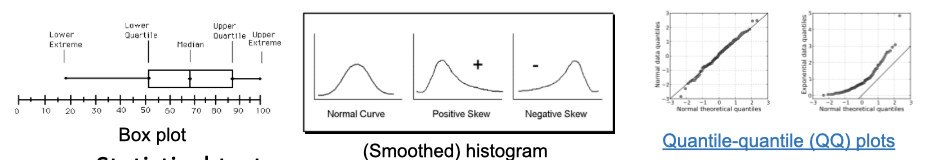
\includegraphics[width=1\textwidth]{plots}
    \label{fig:LABEL}
\end{figure}
\begin{itemize}
	\item Statistical tests:
	\begin{itemize}
		\item Goodness-of-fit tests
		\item Kolmogorov-Smirnoff test
		\item Normality tests
	\end{itemize}
\end{itemize}

\section*{Recognizing a power law}

Use log-log axes, this is the best way to identify it. The result must be a decreasing linear line. 

% Quick centered image
\begin{figure}[H]
    \centering
    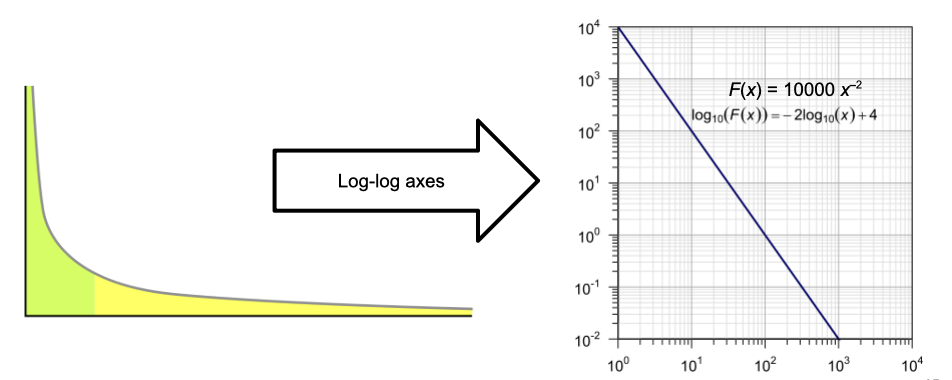
\includegraphics[width=0.8\textwidth]{power-law}
    \label{fig:LABEL}
\end{figure}
\section*{Study case: who likes snickers better?}

% Quick centered image
\begin{figure}[H]
    \centering
    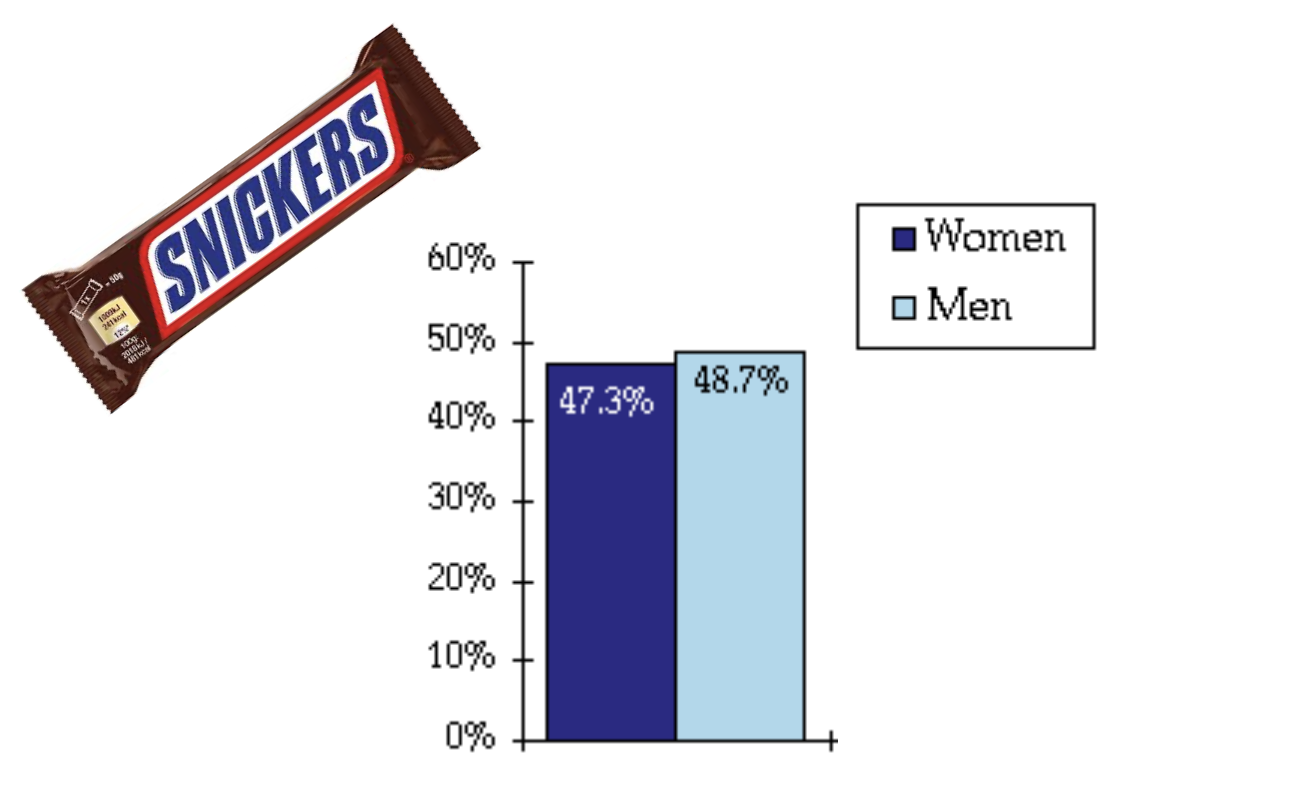
\includegraphics[width=0.6\textwidth]{snickers}
    \label{fig:LABEL}
\end{figure}

\begin{center}
{\LARGE \textbf{Part 2}: Quantifying uncertainty}}
\end{center}

\vspace{1cm}

\begin{itemize}
	\item Most straightforward descriptive statistic to answer this question: mean for each group (women, men)
\end{itemize}

% Quick centered image
\begin{figure}[H]
    \centering
    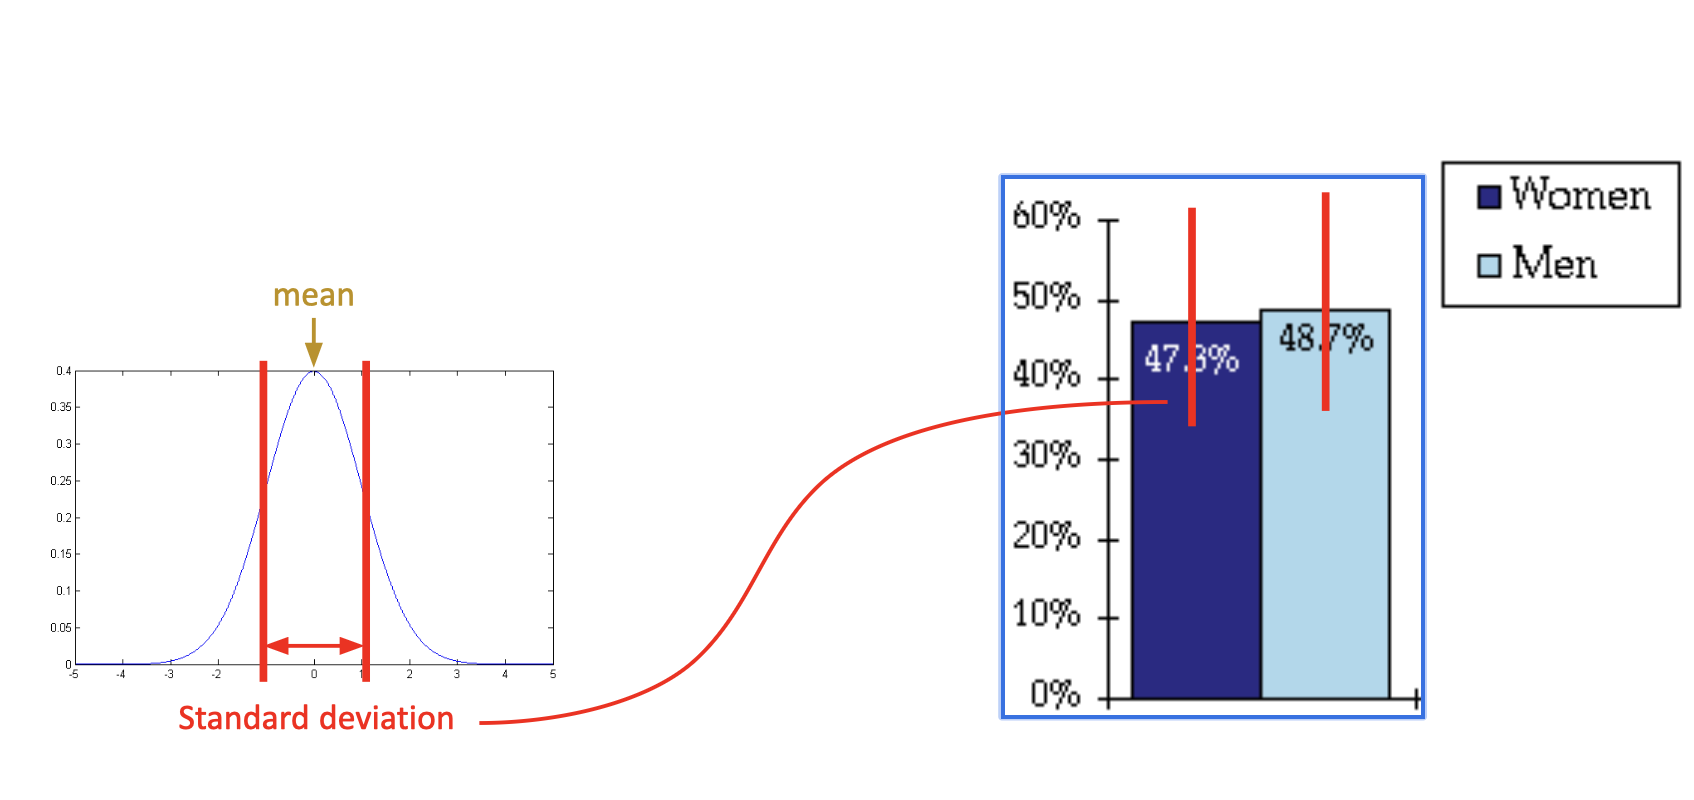
\includegraphics[width=0.7\textwidth]{snickers-mean}
    \label{fig:LABEL}
\end{figure}

\textbf{\textcolor{red}{Always be curtains to quantify your uncertainty!}}

\begin{itemize}
	\item Finite samples introduce uncertainty
		\begin{itemize}
			\item Even a complete dataset is a finite sample!
		\end{itemize}
	\item Whenever you report a statistic, you need to quantify how certain you are in it!
	\item We will discuss two ways of quantifying uncertainty:
	\begin{itemize}
		\item (1) Hypothesis testing
		\item (2) Confidence interval
	\end{itemize}
	\item All plots should have error bars!
\end{itemize}

\section*{How to quantify uncertainty?}
\textbf{Approach 1: Hypothesis testing}

Joseph B. Rhine ran an experiment where subjects had to guess whether 10 hidden cards were red or blue. 

He found that about 1 person in 1000 had ESP ("extrasensory perception"), i.e, they could guess the color of all 10 cards!

Q: Do you agree? $0.5^{10} = 1/1024$ probability to guess correctly!

\textcolor{red}{If there is no real effect, how likely is that I observer data as extreme as I observe?}

\[
	1 - (1 - 2^{-10})^{1000} = 62\%
.\] 

This is the probability of at least someone guess the 10 cards correctly. So it's more likely that someone will guess than no one will guess it. 
He called back the "psychic" subjects and had them do the same test again. They all failed. He concluded that \textbf{the act of telling psychics that they have psychic abilities} causes them to lose...

\textbf{\textcolor{red}{Hypothesis testing}}

\begin{itemize}
	\item A huge subject; can take entire classes on it
	\item Need to understand basics even if you don't use it yourself
	\item Never use it without understanding exactly what you're doing
\end{itemize}

\section*{The logic of hypothesis testing}
\begin{itemize}
	\item Flip a coin 100 times; outcome: 40 heads; "Is the coin fair?"
	\item Null hypothesis: "yes"; alternative hypothesis: "no"
	\item "How likely would I be to see an outcome at least this extreme (i.e., $\leq$ 40 heads) if the null hypothesis were true (i.e., if the coin were fair, i.e., if we expect 500 heads)?
	\item If this probability is large, the null hypothesis suffices to explain the data (and is thus not rejected)
	\item Otherwise, dig deeper in order to understand your data
\end{itemize}

\begin{itemize}
	\item Idea: Gain (weak and indirect) support for a hypothesis \textcolor{blue}{$H_A$} by \textbf{rulling out a null hypothesis} \textcolor{red}{$H_0$}
		\begin{itemize}
			\item \textcolor{red}{$H_0$}: "the coin is fair"(simplest hypothesis)
			\item \textcolor{blue}{$H_A$}: "the coin is not fair (a.k.a. biased)"
		\end{itemize}
\end{itemize}

\begin{itemize}
	\item by inspecting a \textbf{test-statistic}: a measurement made on the data that is likely to be large under \textcolor{blue}{$H_A$} but small under \textcolor{red}{$H_0$}
		\begin{itemize}
			\item e.g., number of heads after 100 coin tosses (1-tailed)
			\item e.g., abs(50 - number of heads after 100 coin tosses) (2-tailed)
		\end{itemize}
\end{itemize}

\section*{Coin example (cont'd)}
\begin{itemize}
	\item \textbf{Null hypothesis} \textcolor{red}{$H_0$}: "the coin is fair", i.e., "probability of heads = 0.5"
	\item \textbf{Test statistic} \textcolor{purple}{s}: abs(50 - # of empirically observed heads after 100 coin tosses)
	\item Pr(S $\mid$ \textcolor{red}{$H_0$}): probability distribution of test statistic, assuming that \textcolor{red}{$H_0$} is true
\end{itemize}


\begin{itemize}
	\item Decision rule: \textbf{reject \textcolor{red}{$H_0$} if Pr(S $\geq$  \textcolor{purple}{s} $\mid$  \textcolor{red}{$H_0$}) $<$ \textcolor{green}{a}},

i.e., if the probability of deviating from 50 heads at least as much as empirically observed is small
\begin{itemize}
	\item Pr(S $\geq$  \textcolor{purple}{s} $\mid$ \textcolor{red}{$H_0$}) = \textbf{"p-value"}
	\item \textcolor{green}{a} = \textbf{"significance level"}
\end{itemize}
\end{itemize}

\begin{itemize}
	\item \textcolor{green}{a} controls "false-rejection rate" (probability of rejecting \textcolor{red}{$H_0$} although it is true)
	\begin{itemize}
		\item You as the data analyst choose \textcolor{green}{a} (common values: 5\%, 1\%, 0.5\%, 0.1\%) 
		\item Higher \textcolor{green}{a} $\Rightarrow$ higher false-rejection rate
	\end{itemize}
		
\end{itemize}

\section*{Selecting the right test}

There are many statistical tests. Although they differ in their details, the basic logic is always the same. The right choice of test depends on multiple factors (here a selection):
\begin{itemize}
	\item Question
	\item Data type (continuous vs. categorical; dimensionality; number of outcomes)
	\item Sample size
	\item When comparing two samples: same population or different population?
	\item Parametric assumptions about distribution of test statistic under null hypothesis? (Less important for large sample size, due to central limit theorem)
\end{itemize}

Good news: \textbf{Plenty of advice available}

\section*{Remarks on p-values}
\begin{itemize}
	\item Widely used in all sciences
	\item They are widely misunderstood!
	\item Don't use them if you don't understand them!
	\item Large p means that even under a simple null hypothesis your data would be quite likely
	\item This tells you nothing about the alternative hypothesis
\end{itemize}

\begin{itemize}
	\item Historically, not means as a method for formally deciding whether a hypothesis is true or not
	\item Rather an informal tool for assessing a particular result
	\item Low p-value means: "The simple null hypothesis doesn't explain the data, so keep looking for other explanations!
	\item p = 0.05 means: if you repeat the experiment 20 times, you'll see extreme data even under null hypothesis $\Rightarrow$ you might have "lucked out"
	\item Look at the effect size ("y-axis"), not just the p-value!
\end{itemize}

\section*{Alternative approach: Bayes factors}

\[
	\frac{Prob(Data, underH_0)}{Prob(Data, under H_A)}
.\] 

\section*{How to quantify uncertainty?}

\textbf{Approach 2: Confidence internals}

\section*{Confidence intervals: idea}
\begin{itemize}
	\item \textcolor{red}{Confidence interval} (CI) = a range of estimates for the parameter of interest (e.g., mean) that seems reasonable given the observed data
	\item Confidence level $\gamma$ $\Rightarrow$ "$\gamma$ CI" (often $\gamma = 95\% \Rightarrow 95\% CI)$
\end{itemize}

\section*{Confidence intervals: definition}

\begin{itemize}
	\item $\mu$: true value of parameter of interest
	\item $m$: empirical estimate of parameter of interest
	\item CIs and hypothesis testing are tightly connected:
		\begin{itemize}
			\item $\gamma$ CI contains values  $\mu_0$ for which the null hypothesis "$H_0: \mu = \mu_0$" cannot be rejected at significance level $1 - \gamma$
		\end{itemize}
\end{itemize}

% Quick centered image
\begin{figure}[H]
    \centering
    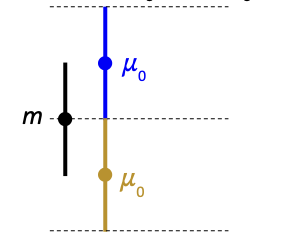
\includegraphics[width=0.3\textwidth]{confidence-intervals}
    \label{fig:LABEL}
\end{figure}

\section*{How to compute confidence intervals?}

\begin{itemize}
	\item \textbf{Parametric} methods assume that the test statistic follows a known (typically Normal) distribution
	$\Rightarrow$ Need to verify that this is actually true! Ugh... 
	\item \textbf{Non-parametric} methods make no assumptions about the distribution of the test statistic. They instead work by sampling the empirical data (Yay!)
\end{itemize}

\section*{Confidence intervals: another view}

\begin{itemize}
	\item If we were to repeat the data collection $N \Rightarrow \infty$ independent times, we'd obtains $N$ estimates of  $\mu : m_1, ..., m_N$
	\item Average of $m_i$'s will approach the true  $\mu$ (by the law of large numbers)
	\item For a fraction  $\gamma$ of the  $N$ repetitions,  $m_i$ lies within the  $\gamma$ CI around  $\mu$
	\item  $\Rightarrow$ May estimate CI from histogram of  $m_i$'s
\end{itemize}
% Quick centered image
\begin{figure}[H]
    \centering
    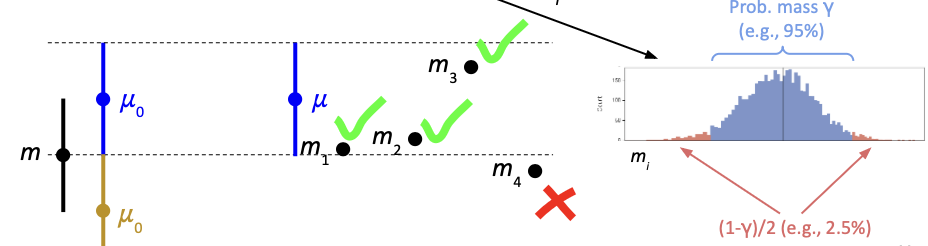
\includegraphics[width=0.8\textwidth]{ci-another-view}
    \label{fig:LABEL}
\end{figure}

\section*{Non-parametric CIs: bootstrap resampling}

% Quick centered image
\begin{figure}[H]
    \centering
    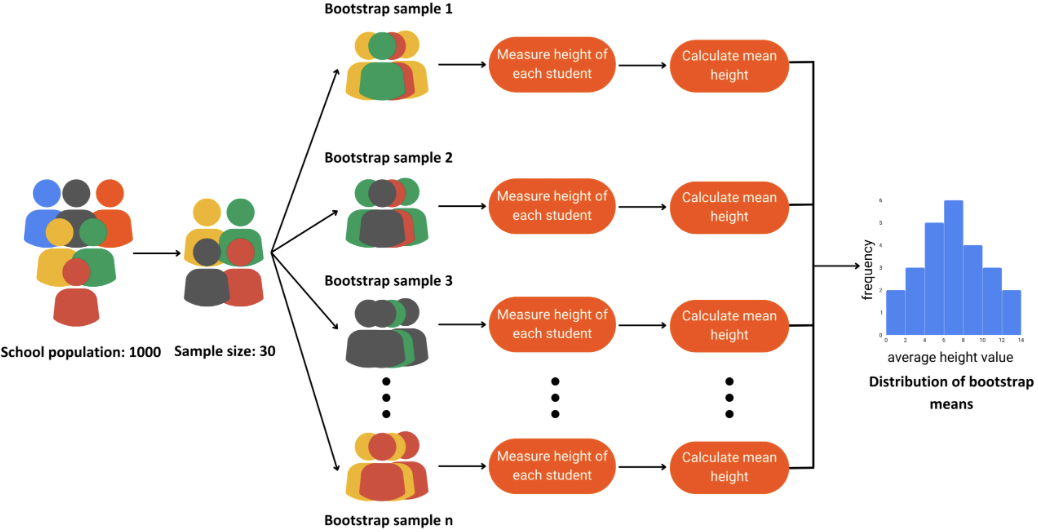
\includegraphics[width=1\textwidth]{bootstrap-resampling}
    \label{fig:LABEL}
\end{figure}

Bootstrap resamples: (random sampling with replacement) $\Rightarrow$ Bootstrap statistics

\section*{Error bars}

\begin{itemize}
	\item An important use case for CIs
	\item But be careful! Error bars can potentially represent many things:
		\begin{itemize}
			\item Confidence intervals (CIs)
			\item Standard deviation
			\item Standard error of the mean: standard deviation/sqrt(n)
		\end{itemize}
	\item Always ask, always tell what the CIs represent!
\end{itemize}

\section*{Multiple-hypothesis testing}

\begin{itemize}
	\item If you perform experiments over and over, you're bound to find something
	\item If you consider "at least one positive outcome" to be the manifestation of an underlying effect: significance level must be adjusted down when performing multiple hypothesis tests!
\end{itemize}

P(detecting an effect when there is none) = $\alpha = 0.05$

P(detecting no effect when there is none) =  $1 - \alpha$

P(detecting no effect when there is none, on every experiment) =  $(1-\alpha)^{k}$
 
P(detecting an effect when there is none \underline{at least one} experiment) = $1 - (1 - \alpha)^{k}$
 
% Quick centered image
\begin{figure}[H]
    \centering
    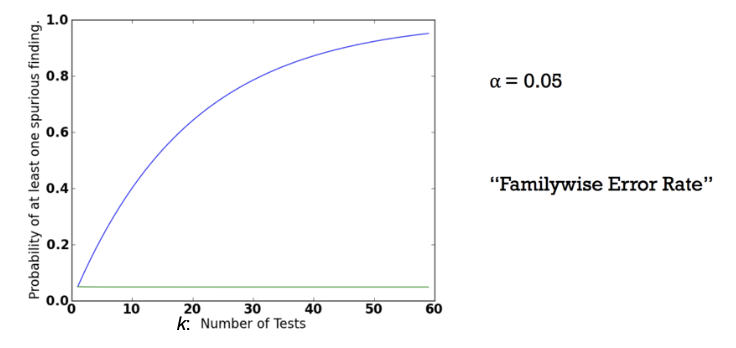
\includegraphics[width=0.7\textwidth]{familiwise-error-rate}
    \label{fig:LABEL}
\end{figure}

\textbf{Bonferroni Correction}
\begin{itemize}
	\item Just divide by the number of hypothesis
	\[
		\alpha_c = \frac{\alpha}{k}
	.\] 
\end{itemize}

\textbf{Sidak Correction}
\begin{itemize}
	\item Asserts independence
	\[
	\alpha = 1 - (1 - \alpha_c)^{k} 
	.\] 
	\[
	 \alpha_c = 1 - (1 - \alpha)^{\frac{1}{k}}
	.\] 
\end{itemize}

\vspace{1cm}
\begin{center}
  {\LARGE \textbf{Part 3}: Relating two variables}
\end{center}

\vspace{1cm}

\section*{Pearson's correlation coefficient}

\begin{itemize}
	\item "Amount of linear dependence"
\end{itemize}

% Quick centered image
\begin{figure}[H]
    \centering
    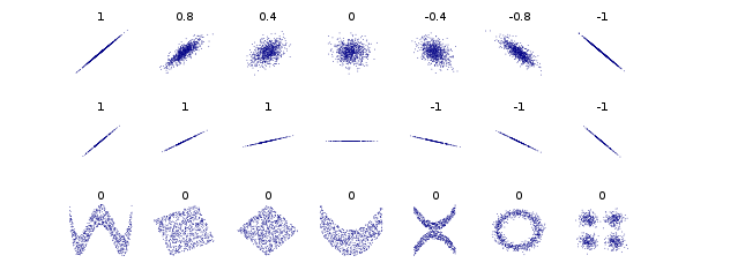
\includegraphics[width=0.9\textwidth]{correlation-coefficient}
    \label{fig:LABEL}
\end{figure}

\textbf{Note}: some of these images are correlated but not linearly correlated...

\begin{itemize}
	\item More general:
		\begin{itemize}
			\item Rank correlation, e.g., Spearman's correlation coefficient
			\item Mutual information
			\item Correlation != causation
		\end{itemize}
\end{itemize}

% Quick centered image
\begin{figure}[H]
    \centering
    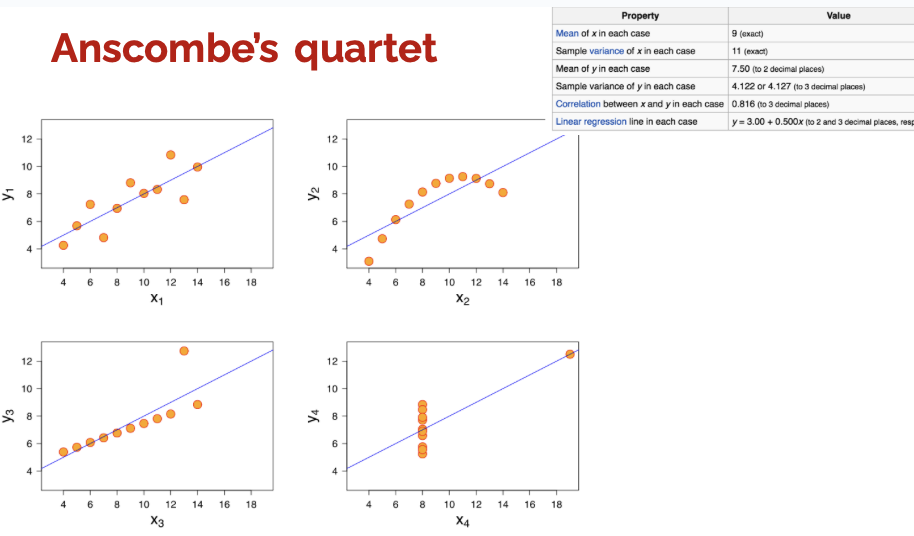
\includegraphics[width=1\textwidth]{anscombe}
    \label{fig:LABEL}
\end{figure}

All different samples are equally correlated!

\section*{UC Berkeley gender bias (?)}

% Quick centered image
\begin{figure}[H]
    \centering
    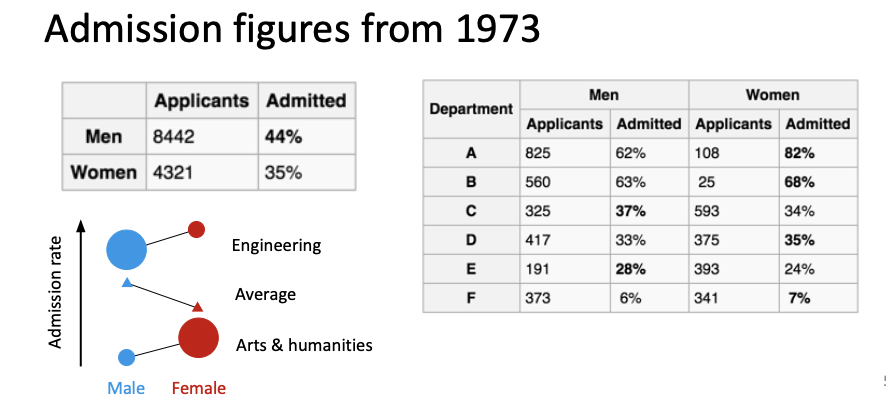
\includegraphics[width=0.8\textwidth]{gender-bias}
    \label{fig:LABEL}
\end{figure}

\section*{Simpson's paradox}

When a trend appears in different groups of data \textbf{but disappears or reverses when these groups are combined} -- beware of aggregates!

In the previous example, \textbf{women tended to apply to competitive departments} with low rates of admission

\end{document}
